
\documentclass[11pt]{article}

%\setlength\topmargin{-0.1in}
%\setlength\headheight{0in}
%\setlength\headsep{0in}
\setlength\textheight{8.5in}
\setlength\textwidth{6.5in}
\setlength\oddsidemargin{0in}
\setlength\evensidemargin{0in}
\usepackage{placeins}
\usepackage{indentfirst}
\usepackage{amsmath}
\usepackage{graphicx}
\usepackage{listings}
\usepackage{rotating}
\usepackage{subcaption} 
\usepackage{booktabs}
\usepackage{tikz}
\usepackage{fancyhdr}
\usepackage{pdfpages}
\usepackage{hyperref}
\usepackage{longtable}
\usepackage[toc,page]{appendix}
%Glossary
\usepackage[acronym,nonumberlist]{glossaries}
\glsaddall %includes all acronymns
%Tables
\usepackage{booktabs}
\newcommand{\ra}[1]{\renewcommand{\arraystretch}{#1}}
%Nomenclature
\usepackage{nomencl}
\makenomenclature
\newif\iffirstglossary\firstglossarytrue
%% This removes the main title:
\renewcommand{\nomname}{}
%% this modifies item separation:
\setlength{\nomitemsep}{15pt}
%% this part defines the groups:
%----------------------------------------------
\usepackage{etoolbox}
\renewcommand\nomgroup[1]{%
  \item[\Large\bfseries
  \ifstrequal{#1}{N}{Nomenclature}{%
  \ifstrequal{#1}{A}{List of Abbreviations}{}}%
]\vspace{10pt}} % this is to add vertical space between the groups.
%----------------------------------------------



\pagestyle{fancy}
\usetikzlibrary{shapes,arrows}
\graphicspath{{Figures/}}
\newcommand{\tabitem}{~~\llap{\textbullet}~~}

\newcommand*{\MyIndent}{\hspace*{0.5cm}}%inerts tab in tables



 
\begin{document} 
\pagenumbering{gobble}

	\begin{titlepage}
	\thispagestyle{empty}
		\newcommand{\HRule}{\rule{\linewidth}{0.5mm}}	
		\center
		\LARGE 
		University of Bath\\
	 	Faculty of Engineering \& Design\\[1cm]	
		%textbf{\Large ME30313 Group Business & Design}\\
		\large
		Word count: XXXXX\\[0.5cm]
		{\large\today}\\[1cm]	
		\HRule\\[0.4cm]	
		{\huge\bfseries Systems Modelling \& Simulation Coursework 1}\\[0.4cm] 	
		\HRule\\[1cm]	
		\begin{minipage}{0.4\textwidth}
			\begin{flushleft}
				\large
				\textit{Supervisor}\\
				A. \textsc{Cookson}
			\end{flushleft}
		\end{minipage}
		~
		\begin{minipage}{0.4\textwidth}
			\begin{flushright}
				\large
				\textit{Assessor}\\
				A. \textsc{Cookson} 
			\end{flushright}
		\end{minipage}\\[1.4cm]
		\large
		\textit{Author}\\
		Xavier \textsc{Forde}\\
		\vfill
		
\includegraphics[width=0.4\textwidth]{UOB_Logo.png}\\
		\vfill 
	\end{titlepage}

%%% ACRONYMS %%

%%END OF ACRONYMS %%%


\thispagestyle{empty}




\tableofcontents
\thispagestyle{empty}
\listoffigures
\listoftables


\nomenclature[A]{CAD}{Computer Aided Design}
\nomenclature[A]{CER}{Cost Estimating Relationship}
\nomenclature[A]{CEF}{Cost Escalation Factor}

\nomenclature[N]{${OWE_{A320}}$}{Operating Weight Empty of the A320}

\printnomenclature


\clearpage
\pagenumbering{arabic}
%\setcounter{page}{1}
\section{Part 1: Software Verification \& Analytical Testing}

\subsection{Derivation of Element Matrix}

Here we will derive the 2-by-2 element matrix for a diffusion operator for an arbitrary element $e_{n}$ between the points $x_{0}$ $x_{1}$. The derivation will start from the weak form version of the diffusion integral, after performing integration by parts. This is given by equation \ref{eq:weakform} in the domain $x = 0$ to $x = 1$.

\begin{equation} \label{eq:weakform}
\int_0^1 D \frac{\partial c}{\partial x}  \frac{\partial v}{\partial x}  dx = \int_0^1 vf dx + \left[vD\frac{\partial c}{\partial x} \right]_0^1
\end{equation}

We have the domain from $x = 0$ to $ x = 1$ which we can split into $ne$ number of elements. This is shown pictorially below for the case $ne = 4$.

%Figure to show elements on a line
\begin{figure}[h!]
\centering
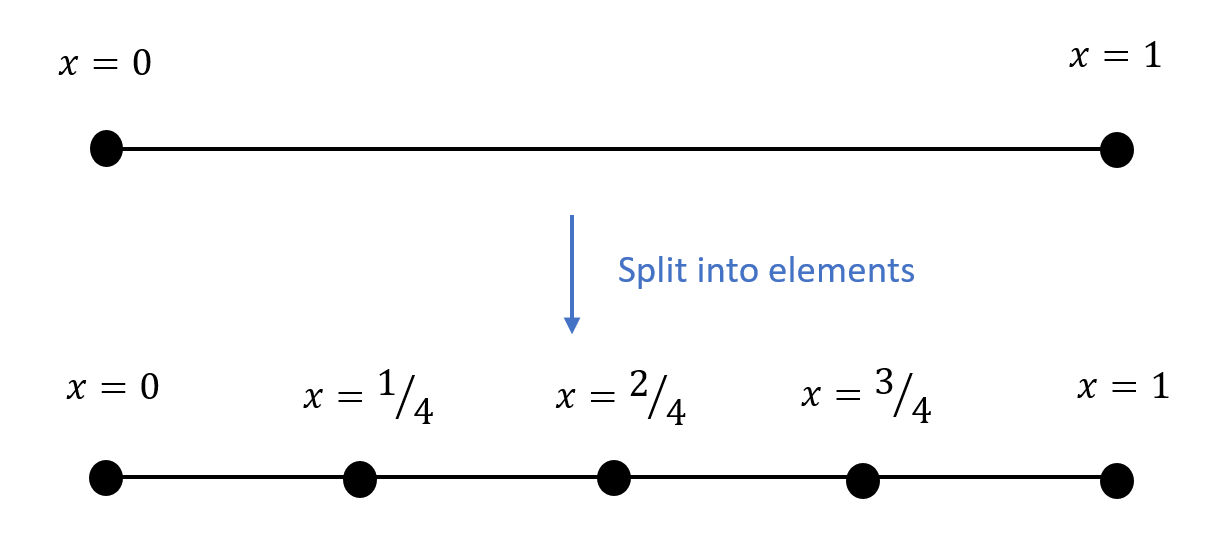
\includegraphics[width=0.75\textwidth]{SplitIntoElements.PNG}
\end{figure}

We can now say the integral from $x = 0$ to $x = 1$ is equivalent to the sum of the integral of the individual elements, for the $ne = 4$ case:


%Splitting Intergral into elements
\begin{equation}
\int_0^1 dx = \int_0^\frac{1}{4}  dx + \int_\frac{1}{4}^\frac{2}{4}  dx + \int_\frac{2}{4}^\frac{3}{4}  dx + \int_\frac{3}{4}^1  dx
\end{equation}

To integrate an individual element we will use linear Lagrange nodal basis function \ref{eq:Lagrange} to represent $c$ and $x$, the functions are shown below. The test function $v$ is set to be equal to the basis function $\psi$.

\begin{subequations}
\label{eq:Lagrange}
\begin{align}
c &= c_{0}\psi_{0}(\zeta) + c_1\psi_{1}(\zeta) \label{eq:LagrangeC} \\
x &= x_{0}\psi_{0}(\zeta) + x_1\psi_{1}(\zeta) \label{eq:LagrangeX} \\
v & = \psi_{0} , \psi_{1} \label{eq:LagrangeV} \\
\text{where,}\\
\psi_{0} &= \frac{1 - \zeta}{2} \ \ \ \ ,  \ \ \ \ \psi_{1} = \frac{1 + \zeta}{2} \label{eq:LagrangePSI}\\
\text{and,}\\
\zeta  & = 2 \left(\frac{x - x_0}{x_1 - x_0}\right) - 1 \label{eq:LagrangeZeta}
\end{align}
\end{subequations}
for $x$ in that element between $x_0$ and $x_1$.\\
We need to map the local element to a standard element as shown below. The Jacobian transform $J$ is used to map from the $x$ to the $\zeta$ coordinate system.

%Local element to standard element
\begin{equation} \label{eq:Jacobian}
J = \left \vert \frac{dx}{d\zeta}\right \vert
\end{equation}



%Figure to show elements mapping to standard
\begin{figure}[h!]
\centering
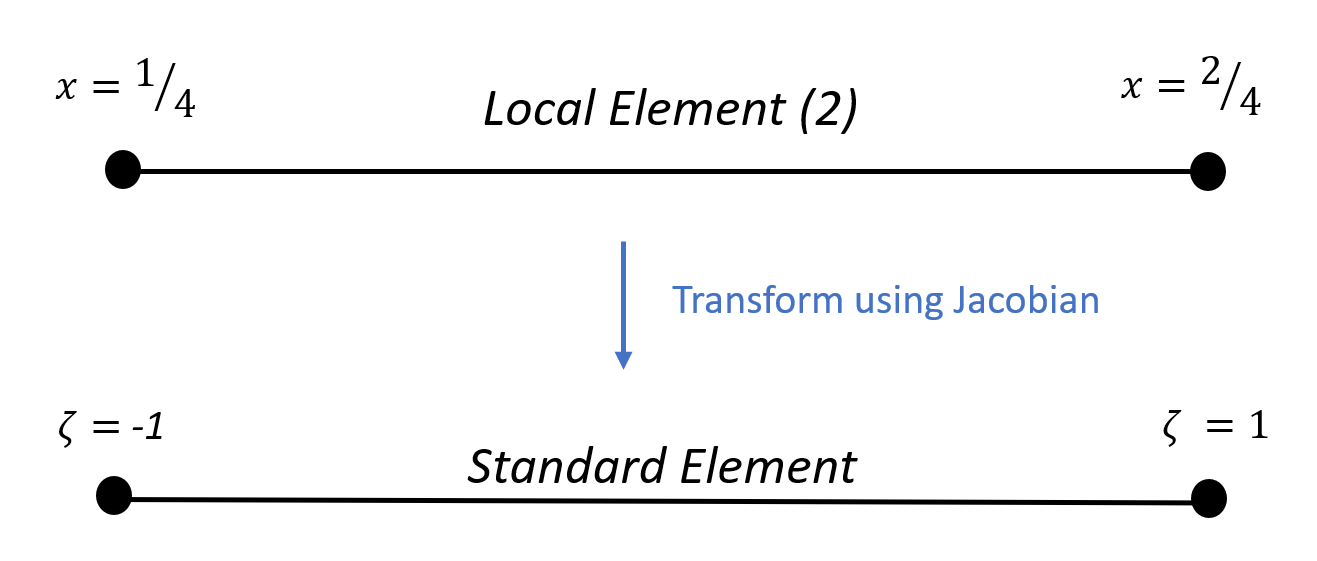
\includegraphics[width=0.75\textwidth]{Local2Standard.PNG}
\end{figure}

Starting with the left hand side of equation \ref{eq:weakform} transforming with the Jacobian to a standard using $dx = Jd\zeta$ we get:

\begin{equation} \label{eq:LHStransform}
\int_{x_0}^{x_{1}} D \frac{\partial c}{\partial x}  \frac{\partial v}{\partial x}  dx =  \int_{-1}^{1} D \frac{\partial c}{\partial x}  \frac{\partial v}{\partial x} J d\zeta
\end{equation}

We need to evaluate the derivatives $\frac{\partial c}{\partial x}$ and $ \frac{\partial v}{\partial x}$ which we can obtain by applying the chain rule to the definitions of c and v given by equations {eq:LagrangeC} and {eq:LagrangeV}. This gives the results

\begin{subequations}
\label{eq:LagrangeD}
\begin{align}
\frac{dc}{dx} &= c_{0}\frac{d\psi_{0}}{d\zeta}\frac{d\zeta}{dx} + c_1\frac{d\psi_{1}}{d\zeta}\frac{d\zeta}{dx} = c_n\frac{d\psi_{n}}{d\zeta}\frac{d\zeta}{dx} \label{eq:LagrangeDC} \ \ \ \text{for} \ n =0,1\\
\frac{dv}{dx} &= \frac{d\psi_{m}}{d\zeta}\frac{d\zeta}{dx} \ \ \ \text{for} \ m =0,1 \label{eq:LagrangeDV} 
\end{align}
\end{subequations}

We can now rewrite equation \ref{eq:LHStransform} as the following, recognising $c$ is independent of $x$ and therefore $\zeta$.
\begin{equation} \label{eq:LHStransform}
 c_n\int_{-1}^{1} D \frac{d\psi_{n}}{d\zeta}\frac{d\zeta}{dx} \frac{d\psi_{m}}{d\zeta}\frac{d\zeta}{dx} J d\zeta
\end{equation}

Knowing that $\frac{d\zeta}{dx} = J^{-1}$ (for $x_1 > x_0$) from equation \ref{eq:Jacobian} and that for a given element $J$ is constant, we can rewrite equation \ref{eq:LHStransform} as

\begin{equation} \label{eq:LHStransform2}
 c_nJ^{-1}\int_{-1}^{1} D \frac{d\psi_{n}}{d\zeta}\frac{d\psi_{m}}{d\zeta} d\zeta \ \ \ \ \text{for} n= 0,1 \& m = 0,1
\end{equation}




From \ref{eq:LHStransform2} we have two equations, one for each node, which when written in full, is clearly suitable for matrix representation.

\begin{subequations}
\label{eq:matrixform}
\begin{align}
&J^{-1} \left  [c_0 \int_{-1}^{1} D \frac{d\psi_{0}}{d\zeta} \frac{d\psi_{0}}{d \zeta} d \zeta + c_1 \int_{-1}^{1} D \frac{d\psi_{1}}{d\zeta} \frac{d\psi_{0}}{d\zeta}d\zeta ) \right ] \label{eq:row1} \\
&J^{-1} \left  [ c_0 \int_{-1}^{1} D \frac{d\psi_{1}}{d\zeta} \frac{d\psi_{0}}{d \zeta} d \zeta + c_1 \int_{-1}^{1} D \frac{d\psi_{1}}{d\zeta} \frac{d\psi_{1}}{d\zeta}d\zeta ) \right ] \label{eq:row2} 
\end{align}
\end{subequations}

The matrix representation is as follows where $I_{nm}$ represents the individual integrals in the above equations \ref{eq:row1} and \ref{eq:row2}. 

%%%	MATRIX Int_nm%%%%%
\begin{equation}
J^{-1}
\begin{bmatrix}

I_{00} & I_{01} \\
I_{10} & I_{11}
\end{bmatrix}
\begin{bmatrix}

c_{0} \\  c_{1} 
\end{bmatrix}
\end{equation}

%%Evaluate integrals%%%%%%%%%
We now need to evaluate each $Int_{nm}$ term individually. In order to evaluate the integrals we need to calculate the derivatives of $\psi_0$ and $\psi_{1}$ with respect to $\zeta$ using the definition of the basis function given by equation \ref{eq:LagrangePSI}. The results is as follows.

\begin{subequations}
\label{eq:prematrix}
\begin{align}
\frac{d\psi_{0}}{d\zeta} &= \frac{d}{d\zeta}(\frac{1-\zeta}{2}) = -\frac{1}{2} \label{eq:psi0der}\\
\frac{d\psi_{1}}{d\zeta} &= \frac{d}{d\zeta}(\frac{1+\zeta}{2}) = \frac{1}{2} \label{eq:psi1der}
\end{align}
\end{subequations}
\\


\underline{$Int_{00}$} \\


\begin{equation}\label{eq:Int00}
\begin{split}
 Int_{00} &= \int_{-1}^{1} D \frac{d\psi_{0}}{d\zeta} \frac{d\psi_{0}}{d \zeta} d \zeta \\
&=  \int_{-1}^{1} D .( -\frac{1}{2}). (-\frac{1}{2}) d\zeta \\
& = \left[ \frac{D}{4} \zeta \right]_{-1}^{1} \\
& = \left[ (\frac{D}{4}.1) - (\frac{D}{4}.-1) \right] \\
& = \frac{D}{2}
\end{split}
\end{equation}

\underline{$Int_{01}$} \\


\begin{equation}\label{eq:Int01}
\begin{split}
 Int_{01} &= \int_{-1}^{1} D \frac{d\psi_{0}}{d\zeta} \frac{d\psi_{1}}{d \zeta} d \zeta \\
&=  \int_{-1}^{1} D .( -\frac{1}{2}). (\frac{1}{2}) d\zeta \\
& = \left[-\frac{D}{4} \zeta \right]_{-1}^{1} \\
& = \left[ (-\frac{D}{4}.1) - (-\frac{D}{4}.-1) \right] \\
& = -\frac{D}{2}
\end{split}
\end{equation}

\underline{$Int_{10}$} \\


\begin{equation}\label{eq:Int10}
\begin{split}
 Int_{01} &= \int_{-1}^{1} D \frac{d\psi_{1}}{d\zeta} \frac{d\psi_{0}}{d \zeta} d \zeta \\
&=  \int_{-1}^{1} D .( \frac{1}{2}). (-\frac{1}{2}) d\zeta \\
& = \left[-\frac{D}{4} \zeta \right]_{-1}^{1} \\
& = \left[ (-\frac{D}{4}.1) - (-\frac{D}{4}.-1) \right] \\
& = -\frac{D}{2}
\end{split}
\end{equation}


\clearpage

\underline{$Int_{11}$} \\


\begin{equation}\label{eq:Int11}
\begin{split}
 Int_{11} &= \int_{-1}^{1} D \frac{d\psi_{1}}{d\zeta} \frac{d\psi_{1}}{d \zeta} d \zeta \\
&=  \int_{-1}^{1} D .( \frac{1}{2}). (\frac{1}{2}) d\zeta \\
& = \left [\frac{D}{4} \zeta \right ]_{-1}^{1} \\
& = \left [ (\frac{D}{4}.1) - (\frac{D}{4}.-1) \right ] \\
& = \frac{D}{2}
\end{split}
\end{equation}

We can now assemble our local element matrix (not including the c term matrix). This is the form used in the code for LaplaceElemMatrix.m function. Where J and D are scalars (we have assumed D to be constant).

%%%	Final MATRIX Int_nm%%%%%
\begin{equation}
J^{-1}D
\begin{bmatrix}

0.5 & -0.5 \\
-0.5 & 0.5
\end{bmatrix}
\end{equation}


\section{Conclusions}










\pagebreak



%\begin{thebibliography}{9}
%%Last name, First Initial, Year published. Title. Publisher, Volume, Page(s).
%% HARVARD REFERENCE STYLE:
%%Brunner, F.H., 1949. Synthetic gasoline from natural gas. Industrial and engineering chemistry, 41(11), pp.2511-2515.
%
%\bibitem{SPEC} 
%Macgregor, K., 2017. 
%\textit{Student Design Project Specification 2017/18.}
%Airbus Group.
%
%\bibitem{CS25} 
%European Aviation Safety Agency (EASA), 2007.
%\textit{Certification Specifications for Large Aeroplanes: CS-25. Amendment 3.}
%
%\bibitem{Sherman} 
%Sherman, D., 2009.
%\textit{Systems Cost Engineering: Affordability Management and Cost Control.}
%
%\bibitem{pwc}
%Thisdell, D. 2015.
%\textit{Top 100 Report.}
%Flight International 2014. 
%
%\bibitem{kit}
%Thornton, K., 2018.
%\textit{Phase 3 Secondary Report: DOC.}
%University of Bath: CTA1 – Aerospace Group Business \& Design Project II.
%
%\bibitem{ben}
%Earl, B., 2018.
%\textit{Phase 3 Secondary Report: Marketing.}
%University of Bath: CTA1 – Aerospace Group Business \& Design Project II.
%
%\bibitem{jenk}
%Jenkinson. L.R., 1999.
%\textit{Civil Jet Aircraft Design.}
%Butterworth-Heinemann.
%
%\bibitem{josht}
%Bowen, J. 2018.
%\textit{Phase 3 Primrary Report: Propulsion.}
%University of Bath: CTA1 – Aerospace Group Business \& Design Project II.
%
%\bibitem{R5}
%Roskam, J., 1985.
%\textit{Airplane Design Part V: Component Weight Estimation.}
%The University of Kansas.
%
%\bibitem{R8}
%Roskam, J., 1985.
%\textit{Airplane Design Part VIII: Airplane Cost Estimation: Design, Development, Manufacturing and Operating.}
%The University of Kansas.
%
%\bibitem{ATRPROD}
%http://rzjets.net/aircraft/?page=25\&typeid=310
%
%\bibitem{jane}
%P. Jackson et al, 2013.
%\textit{JANE'S ALL THE WORLD'S AIRCRAFT.}
% 
%
%\bibitem{Raymer}
%Raymer, D.P., 1992.
%\textit{Aircraft Design: A Conceptual Approach.}
%AIAA Education Series. 
%
%\bibitem{RAND}
%Hess, R. W. and Romanoff, H.P., 1987.
%\textit{Aircraft Airframe Cost Estimating Relationships.}
%Rand Corp. 
%
%\bibitem{MARKISH}
%Markish, J., 1987.
%\textit{Valuation Techniques for Commercial Aircraft Program Design.}
%Massachusetts Institute of Technology.
%
%\bibitem{PW150}
%Forecast International, 2010.
%\textit{The Market For Turboprop Engines.}
%Forecast International.
%
%\bibitem{reuters}
%Hepher, T., 2017.
%\textit{Turboprop planemaker ATR says demand sufficient to keep production stable.}
%Reuters, available: https://uk.reuters.com/article/us-airbus-leonardo-atr/turboprop-planemaker-atr-says-demand-sufficient-to-keep-production-stable-idUKKCN1BO1IA
%
%\bibitem{discount}
%Schonland, A., 2016.
%\textit{https://airinsight.com/aircraft-pricing-list-vs-market/}
%
%\bibitem{CESNA}
%Eastlake, C.N \& Blackwell, H.W., 
%\textit{Cost Estimating Software for General Aviation Aircraft Design.}
%Embry-Riddle Aeronautical University/Lockheed Martin Corporation.
%
%\bibitem{a320}Zhang, B., 2015.
%\textit{Check out the \$600-million Airbus factory in Alabama — where planes will be built for America.}
%Business Insider.
%
%\bibitem{becky}
%Leach, B., 2018.
%\textit{Phase 3 Secondary Report: Management Strategy for Final Assembly}
%University of Bath: CTA1 – Aerospace Group Business \& Design Project II.
%
%\bibitem{IRR}
%Dressel, C., 2018.
%\textit{Project Costing \& Business Case}
%Airbus Group.


%\end{thebibliography}

%\pagebreak
%
%\begin{appendices}
%\section{Cash Flow Statement}
%
%\begin{figure}[p]  %nrcVrc Figure
%	\centering
%	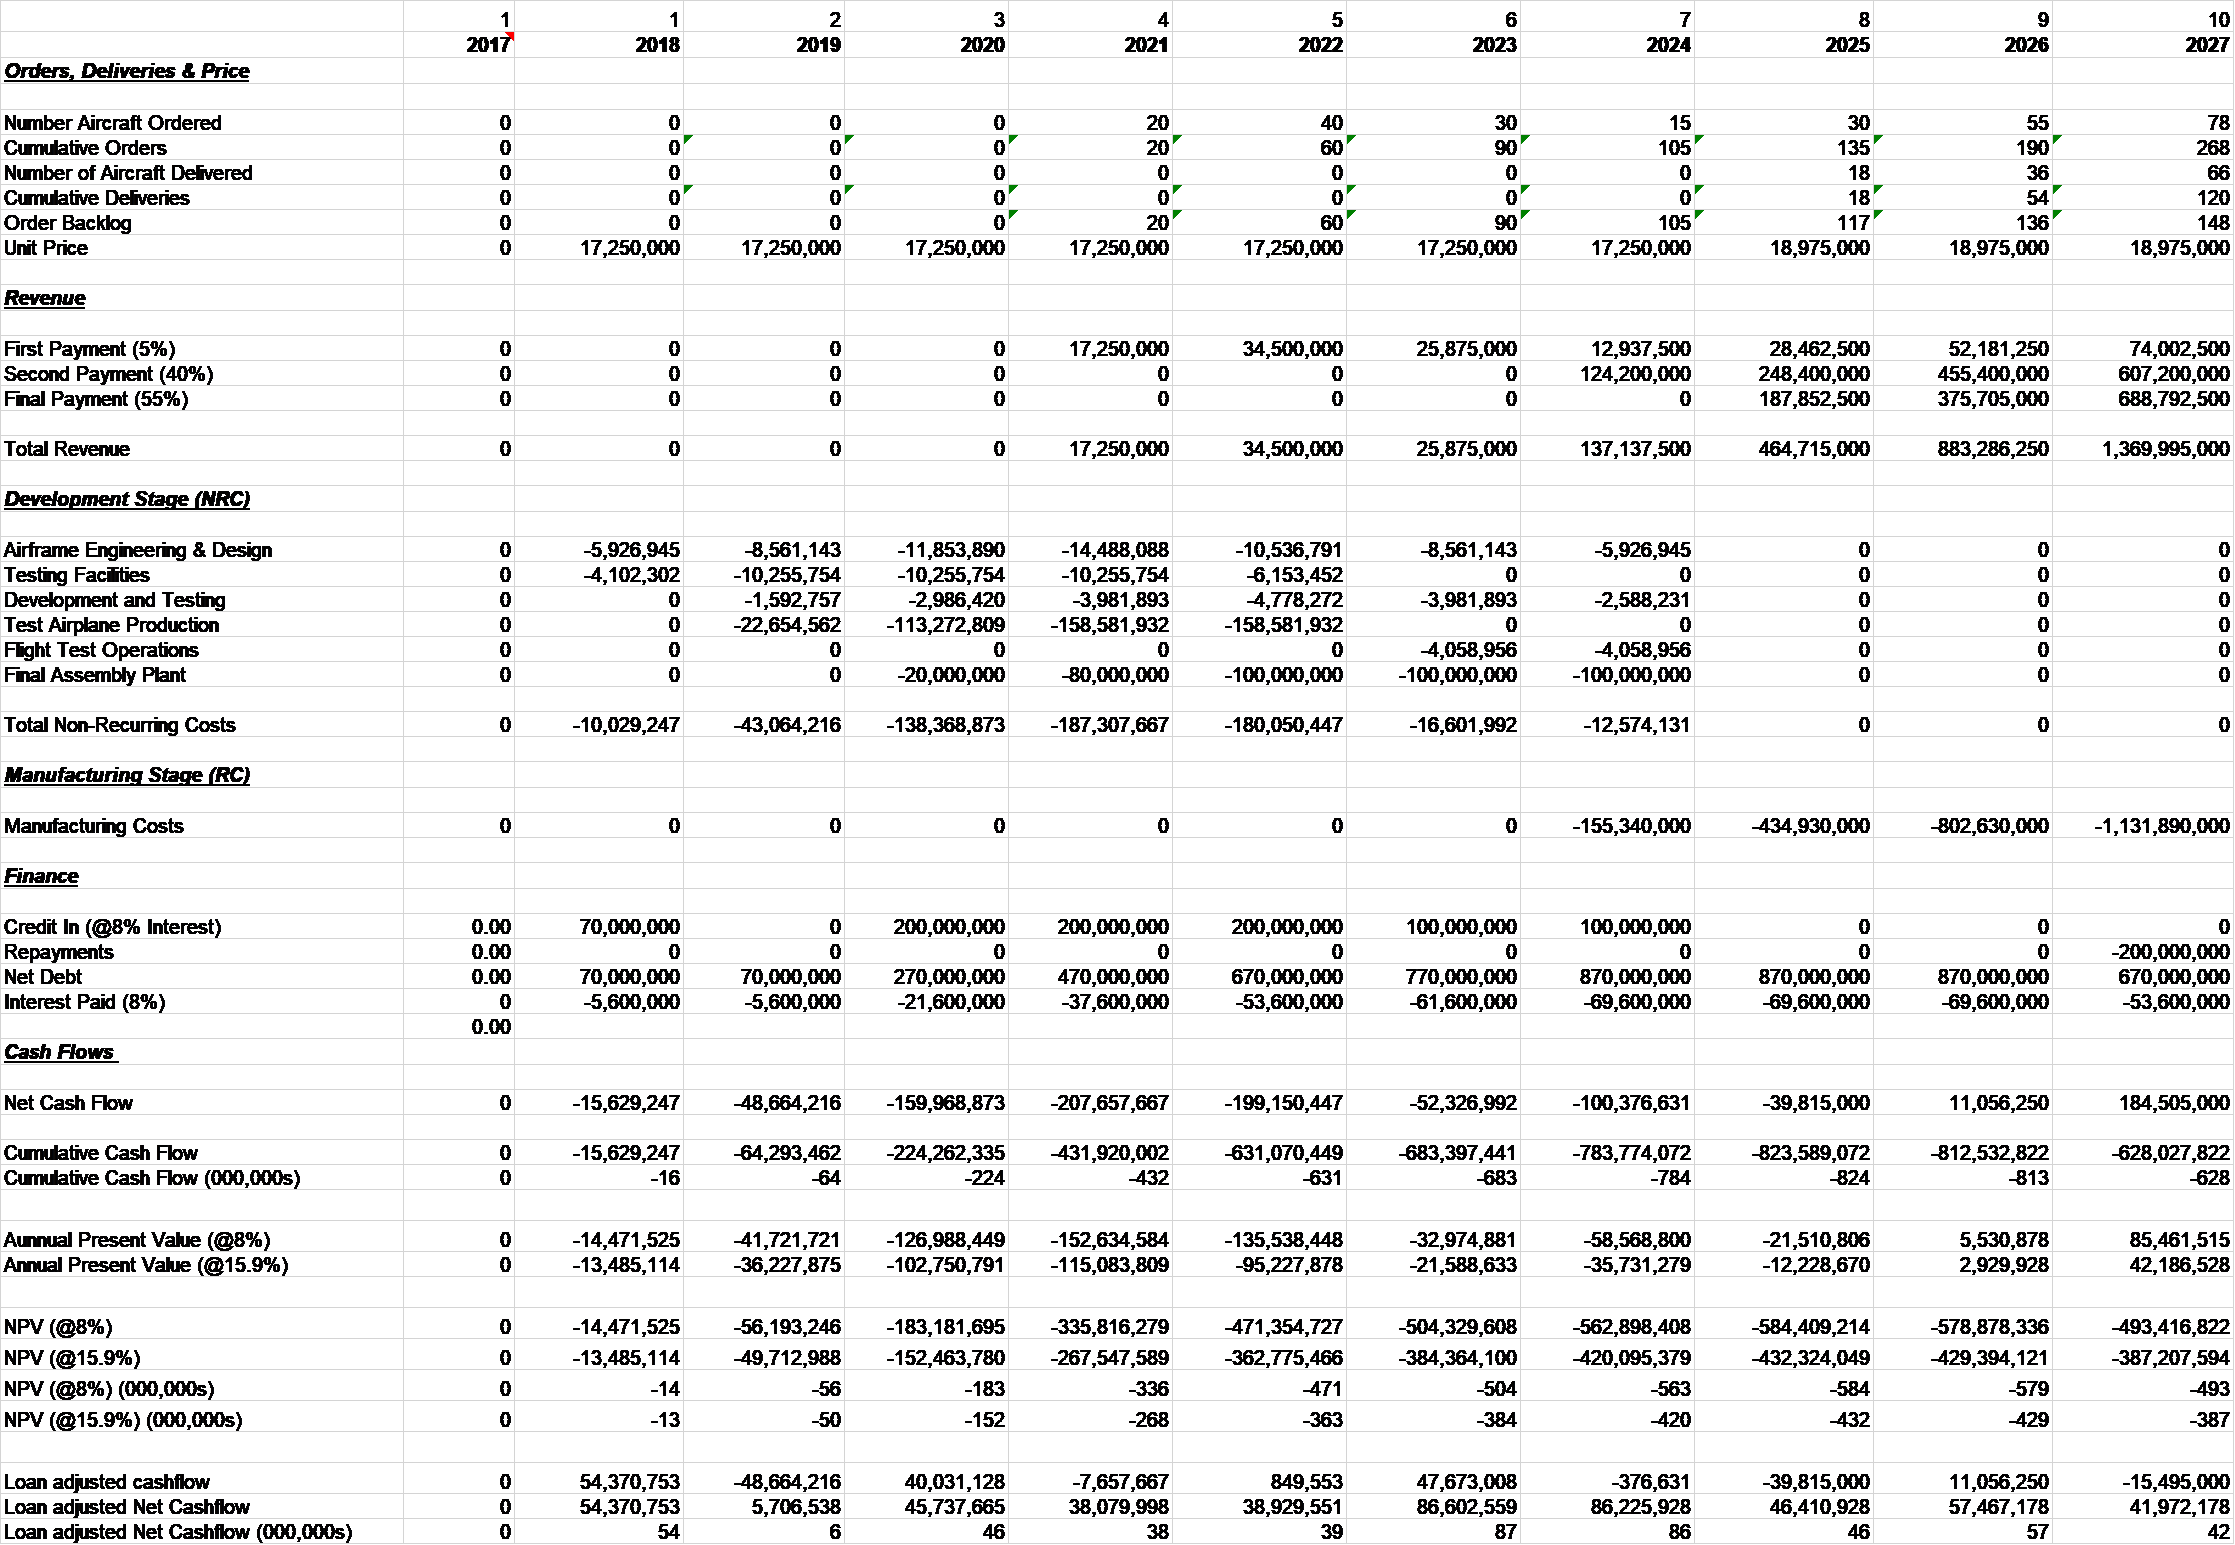
\includegraphics[width=1.2\textwidth, angle=270]{cashflow1.png}
%\end{figure} 
%
%\begin{figure}[p]  %nrcVrc Figure
%	\centering
%	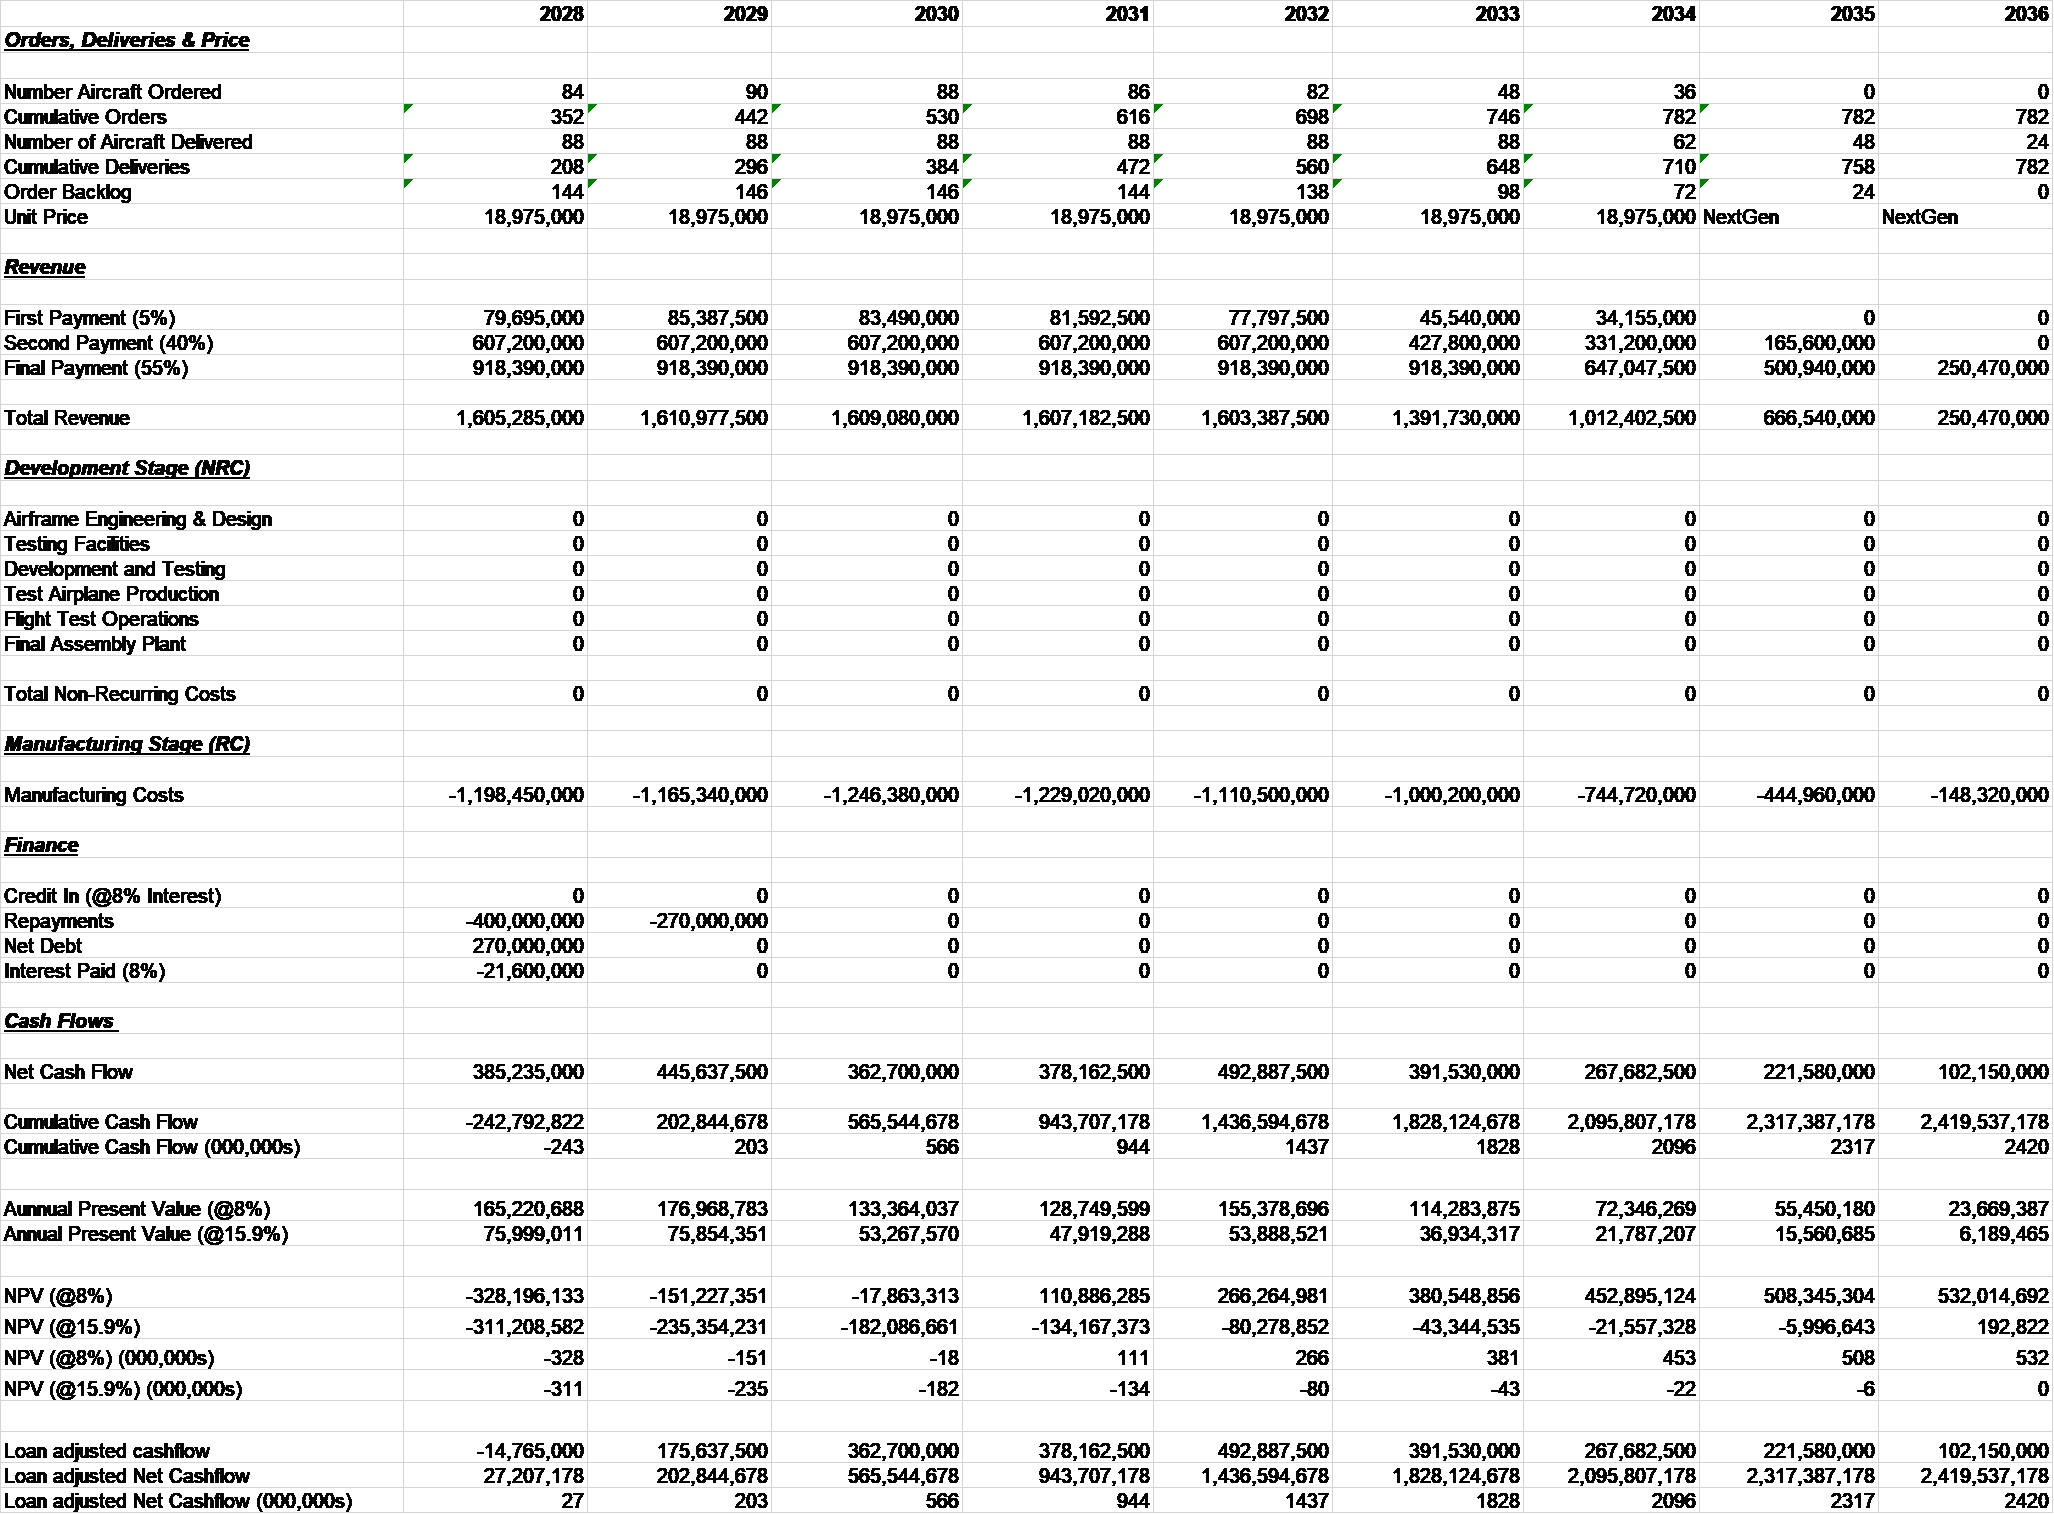
\includegraphics[width=1.2\textwidth, angle=270]{cashflow2.png}
%\end{figure} 
%
%\pagebreak
%\section{General Arrangement Drawing}
%\end{appendices}





\end{document}

